% Master test document for visual inspection of all paper figures.
% Compiles all 9 figures in sequence as a single PDF. Drop into NeurIPS
% style file by inputting individual \input{fig_*} files in the paper.
%
%   pdflatex figures_master.tex
%   pdflatex figures_master.tex  % twice for cross-references
%
\documentclass[11pt]{article}
\usepackage[margin=0.75in]{geometry}
\usepackage{tikz}
\usepackage{pgfplots}
\pgfplotsset{compat=1.18}
\usetikzlibrary{
  arrows.meta,
  positioning,
  shapes.geometric,
  decorations.pathreplacing,
  calc
}
\usepackage{caption}
\usepackage{booktabs}
\captionsetup{font=small, labelfont=bf}

\title{Discovery Tetrad — Paper Figures (Master Test File)}
\author{(authors redacted for double-blind review)}
\date{\today}

\begin{document}
\maketitle

\noindent This document compiles all 9 paper figures for visual inspection.
Each figure is also available as a standalone \texttt{.tex} fragment in
\texttt{paper/figures/}; the paper input order is:

\begin{enumerate}\itemsep0pt
  \item \texttt{fig\_substrate\_inheritance.tex} — \S 4 setup overview.
  \item \texttt{fig\_pipeline.tex} — \S 4 pipeline architecture.
  \item \texttt{fig\_tetrad\_arch.tex} — \S 3 four-gate two-layer architecture.
  \item \texttt{fig\_cell\_taxonomy.tex} — \S 3 25-cell verdict taxonomy.
  \item \texttt{fig\_cascade.tex} — \S 3 witness-layer cascade rule.
  \item \texttt{fig\_witness\_loop.tex} — \S 3 iterative re-evaluation.
  \item \texttt{fig\_goal\_witness\_failure.tex} — \S 1 case study (compreg).
  \item \texttt{fig\_sophism\_density.tex} — \S 5 headline result.
  \item \texttt{fig\_cell\_heatmap.tex} — \S 5 cell occupancy across substrates.
  \item \texttt{fig\_concordance.tex} — Appendix three-way concordance.
\end{enumerate}

\clearpage
% Substrate inheritance / provenance overview.
% Designed for full text-width.
\begin{figure}[t]
\centering
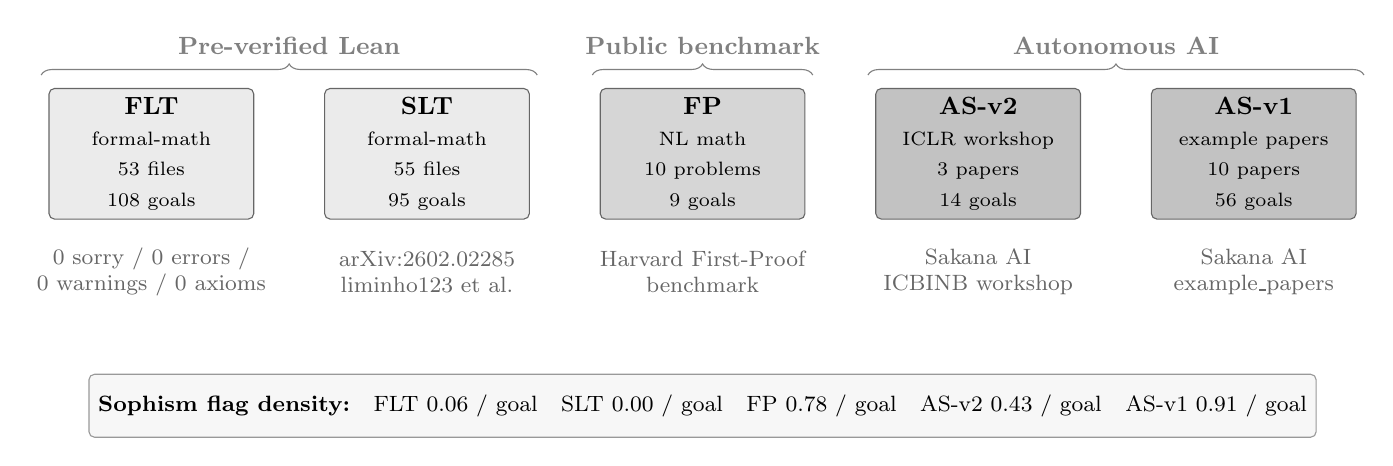
\begin{tikzpicture}[
  font=\small,
  substrate/.style={
    rectangle, rounded corners=2pt, draw=black!60,
    minimum width=2.6cm, minimum height=1.6cm, align=center
  },
  formal/.style={substrate, fill=black!8},
  empirical/.style={substrate, fill=black!16},
  ai/.style={substrate, fill=black!24},
  brace/.style={decorate, decoration={brace, amplitude=4pt}, black!50},
  flow/.style={-{Latex[length=2mm]}, black!70, line width=0.5pt, dashed},
]

% Five substrates in a row
\node[formal] (flt) at (-7.0, 0)
  {\textbf{FLT}\\\scriptsize formal-math\\\scriptsize 53 files\\\scriptsize 108 goals};
\node[formal] (slt) at (-3.5, 0)
  {\textbf{SLT}\\\scriptsize formal-math\\\scriptsize 55 files\\\scriptsize 95 goals};
\node[empirical] (fp) at (0, 0)
  {\textbf{FP}\\\scriptsize NL math\\\scriptsize 10 problems\\\scriptsize 9 goals};
\node[ai] (asv2) at (3.5, 0)
  {\textbf{AS-v2}\\\scriptsize ICLR workshop\\\scriptsize 3 papers\\\scriptsize 14 goals};
\node[ai] (asv1) at (7.0, 0)
  {\textbf{AS-v1}\\\scriptsize example papers\\\scriptsize 10 papers\\\scriptsize 56 goals};

% Group labels (above)
\draw[brace] (-8.4, 1.0) -- (-2.1, 1.0)
  node[midway, above=4pt, font=\small\bfseries] {Pre-verified Lean};
\draw[brace] (-1.4, 1.0) -- (1.4, 1.0)
  node[midway, above=4pt, font=\small\bfseries] {Public benchmark};
\draw[brace] (2.1, 1.0) -- (8.4, 1.0)
  node[midway, above=4pt, font=\small\bfseries] {Autonomous AI};

% Provenance row
\node[font=\footnotesize, black!60, align=center] at (-7.0, -1.5)
  {0 sorry / 0 errors / \\ 0 warnings / 0 axioms};
\node[font=\footnotesize, black!60, align=center] at (-3.5, -1.5)
  {arXiv:2602.02285 \\ liminho123 et al.};
\node[font=\footnotesize, black!60, align=center] at (0, -1.5)
  {Harvard First-Proof \\ benchmark};
\node[font=\footnotesize, black!60, align=center] at (3.5, -1.5)
  {Sakana AI \\ ICBINB workshop};
\node[font=\footnotesize, black!60, align=center] at (7.0, -1.5)
  {Sakana AI \\ example\_papers};

% Discriminative axis annotation (below)
\node[align=center, font=\footnotesize, draw=black!40, fill=black!3,
      rounded corners=2pt, minimum width=14cm, minimum height=0.8cm] at (0, -3.2)
  {\textbf{Sophism flag density:}\quad
   FLT 0.06 / goal\quad SLT 0.00 / goal\quad
   FP 0.78 / goal\quad AS-v2 0.43 / goal\quad AS-v1 0.91 / goal};

\end{tikzpicture}
\caption{Substrate inheritance and provenance. The five substrates span three
qualitatively different artifact types: pre-verified clean Lean
formalizations (FLT, SLT), a public natural-language mathematical research
benchmark (FP), and autonomous-AI-generated paper artifacts (AS-v2, AS-v1).
Goal-counts are the dataset's per-substrate population. The sophism-flag
density annotated at the bottom is the headline discriminative result.}
\label{fig:substrate_inheritance}
\end{figure}

% Pipeline architecture: dispatch -> orchestrator -> judge -> output -> validation+aggregation.
% Designed for full text-width.
\begin{figure}[t]
\centering
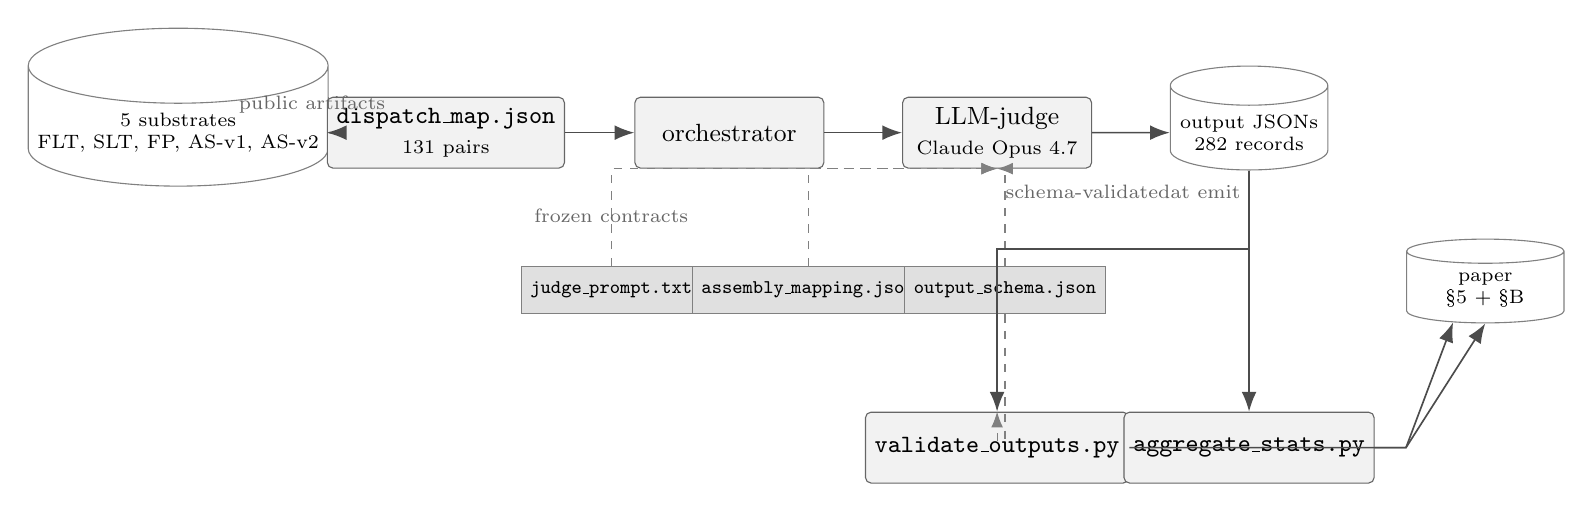
\begin{tikzpicture}[
  font=\small,
  block/.style={
    rectangle, rounded corners=2pt, draw=black!60, fill=black!5,
    minimum width=2.4cm, minimum height=0.9cm, align=center
  },
  contract/.style={
    rectangle, draw=black!50, fill=black!12,
    minimum width=2.0cm, minimum height=0.6cm, align=center,
    font=\scriptsize
  },
  data/.style={
    cylinder, shape border rotate=90, aspect=0.25,
    draw=black!50, fill=white, minimum width=2.0cm, minimum height=1.0cm,
    align=center, font=\scriptsize
  },
  flow/.style={-{Latex[length=2.5mm]}, black!70, line width=0.6pt},
  contractflow/.style={-{Latex[length=2mm]}, dashed, black!50, line width=0.4pt},
]

% Top row: substrate sources
\node[data] (sub) at (0, 1.6) {5 substrates\\\scriptsize FLT, SLT, FP, AS-v1, AS-v2};

% Dispatch map
\node[block] (disp) at (3.4, 1.6) {\texttt{dispatch\_map.json}\\\scriptsize 131 pairs};

% Orchestrator
\node[block] (orch) at (7.0, 1.6) {orchestrator};

% Judge
\node[block] (judge) at (10.4, 1.6) {LLM-judge\\\scriptsize Claude Opus 4.7};

% Outputs
\node[data] (out) at (13.6, 1.6) {output JSONs\\\scriptsize 282 records};

% Frozen contracts (middle row, feed into judge)
\node[contract] (jp)  at (5.5, -0.4) {\texttt{judge\_prompt.txt}};
\node[contract] (am)  at (8.0, -0.4) {\texttt{assembly\_mapping.json}};
\node[contract] (os)  at (10.5, -0.4) {\texttt{output\_schema.json}};

% Bottom row: post-processing
\node[block] (val)   at (10.4, -2.4) {\texttt{validate\_outputs.py}};
\node[block] (agg)   at (13.6, -2.4) {\texttt{aggregate\_stats.py}};
\node[data]  (paper) at (16.6, -0.4) {paper\\\scriptsize\S5 + \S B};

% Top-row flows
\draw[flow] (sub) -- (disp);
\draw[flow] (disp) -- (orch);
\draw[flow] (orch) -- (judge);
\draw[flow] (judge) -- (out);

% Contracts feed into judge
\draw[contractflow] (jp.north) -- (jp |- judge.south) -- (judge.south);
\draw[contractflow] (am.north) -- (am |- judge.south) -- (judge.south);
\draw[contractflow] (os.north) -- (os |- judge.south) -- (judge.south);

% Outputs flow down to validator + aggregator
\draw[flow] (out.south) -- ++(0,-1.0) -| (val.north);
\draw[flow] (out.south) -- ++(0,-1.0) -| (agg.north);

% Validator/aggregator -> paper
\draw[flow] (val.east) -- (val.east -| paper.west) -- (paper.south west);
\draw[flow] (agg.east) -- (agg.east -| paper.west) -- (paper.south);

% Schema validates outputs
\draw[contractflow] (os.south) -- ++(0,-1.6) -| (val.north);

% Annotations
\node[font=\scriptsize, black!60, align=center] at (5.5, 0.55)
  {frozen contracts};
\node[font=\scriptsize, black!60] at (1.7, 1.95) {public artifacts};
\node[font=\scriptsize, black!60] at (12.0, 0.85) {schema-validated\\at emit};

\end{tikzpicture}
\caption{Audit pipeline. A locked dispatch map enumerates 131 (goal-source,
witness) pairs across five substrates. The orchestrator hands each pair to
the LLM-judge under three frozen contracts (the prompt, the verdict-bits to
cell-label assembly mapping, and the output JSON Schema). The judge emits one
schema-valid record per identified goal. Post-processing scripts validate
schema and cascade conformance and produce the cross-substrate aggregates
that drive the empirical-results section. The judge instrument is uniform
across all five substrates.}
\label{fig:pipeline}
\end{figure}

% Discovery Tetrad architecture: 4 gates × 2 layers + cascade asymmetry.
% Designed for full text-width in NeurIPS two-column layout.
\begin{figure}[t]
\centering
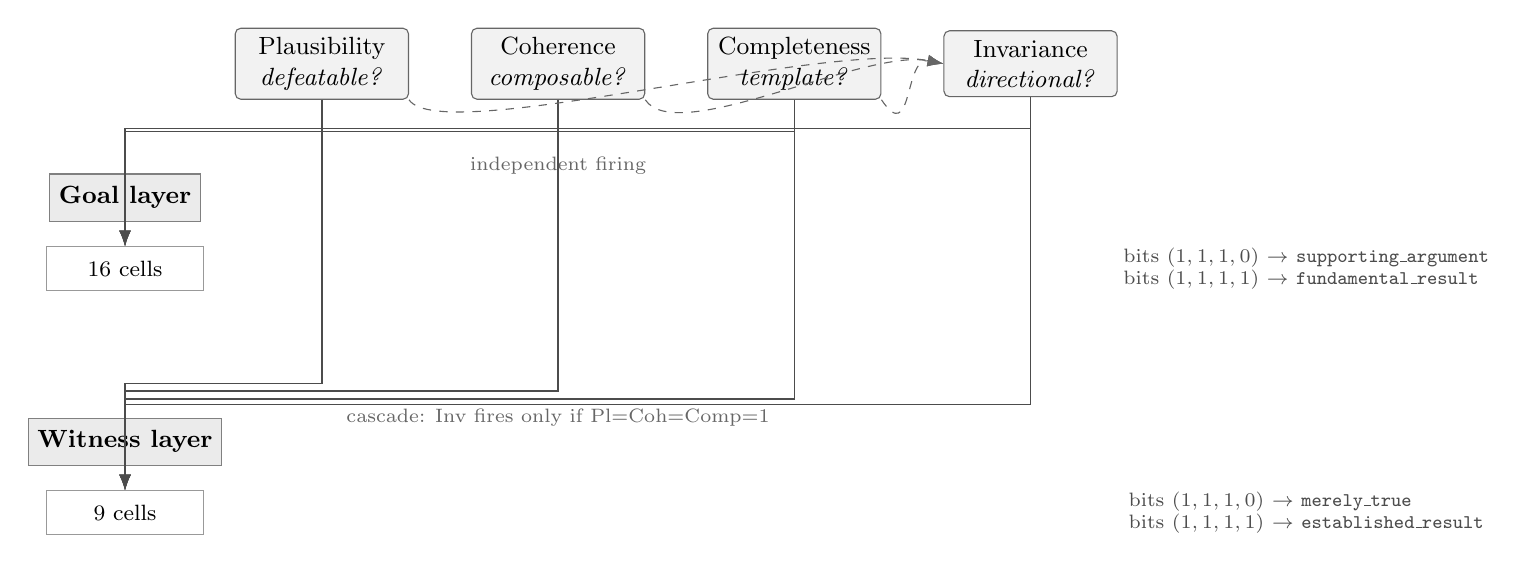
\begin{tikzpicture}[
  font=\small,
  gate/.style={
    rectangle, rounded corners=2pt, draw=black!60, fill=black!5,
    minimum width=2.2cm, minimum height=0.8cm, align=center
  },
  layerlbl/.style={
    rectangle, draw=black!50, fill=black!8,
    minimum width=1.8cm, minimum height=0.6cm, align=center
  },
  cellbox/.style={
    rectangle, draw=black!40, fill=white,
    minimum width=2.0cm, minimum height=0.55cm, align=center,
    font=\footnotesize
  },
  cascadearrow/.style={
    -{Latex[length=2mm]}, dashed, black!60, line width=0.4pt
  },
  feed/.style={-{Latex[length=2mm]}, black!70, line width=0.5pt},
]

% Gates (top row)
\node[gate] (pl)   at (0,0)   {Plausibility \\ \textit{defeatable?}};
\node[gate] (coh)  at (3,0)   {Coherence \\ \textit{composable?}};
\node[gate] (comp) at (6,0)   {Completeness \\ \textit{template?}};
\node[gate] (inv)  at (9,0)   {Invariance \\ \textit{directional?}};

% Goal layer (left side)
\node[layerlbl] (goal) at (-2.5, -1.7) {\textbf{Goal layer}};
\node[cellbox] (gout) at (-2.5, -2.6) {16 cells};

% Goal layer arrows (independent firing — solid arrows from each gate)
\foreach \g in {pl, coh, comp, inv} {
  \draw[feed] (\g.south) -- ++(0,-0.4) -| (gout.north);
}
\node[font=\scriptsize, black!60] at (3, -1.3) {independent firing};

% Witness layer (right side, lower)
\node[layerlbl] (wit) at (-2.5, -4.8) {\textbf{Witness layer}};
\node[cellbox] (wout) at (-2.5, -5.7) {9 cells};

% Witness layer cascade: Pl/Coh/Comp fire, Inv depends on them
\draw[feed] (pl.south)   -- ++(0,-3.6) -| (wout.north);
\draw[feed] (coh.south)  -- ++(0,-3.7) -| (wout.north);
\draw[feed] (comp.south) -- ++(0,-3.8) -| (wout.north);

% Cascade dependency: Pl/Coh/Comp -> Inv (dashed)
\draw[cascadearrow] (pl.south east)   .. controls +(0.4,-0.6) and +(-1.5,0.3) .. (inv.west);
\draw[cascadearrow] (coh.south east)  .. controls +(0.4,-0.6) and +(-1.0,0.2) .. (inv.west);
\draw[cascadearrow] (comp.south east) .. controls +(0.4,-0.6) and +(-0.5,0.1) .. (inv.west);

\draw[feed] (inv.south) -- ++(0,-3.9) -| (wout.north);

\node[font=\scriptsize, black!60] at (3, -4.5)
  {cascade: Inv fires only if Pl=Coh=Comp=1};

% Cells 8/9 layer-specialization annotation
\node[font=\scriptsize, align=left, black!70] at (12.5, -2.6)
  {bits $(1,1,1,0)$ $\to$ \texttt{supporting\_argument}\\
   bits $(1,1,1,1)$ $\to$ \texttt{fundamental\_result}};
\node[font=\scriptsize, align=left, black!70] at (12.5, -5.7)
  {bits $(1,1,1,0)$ $\to$ \texttt{merely\_true}\\
   bits $(1,1,1,1)$ $\to$ \texttt{established\_result}};

\end{tikzpicture}
\caption{The Discovery Tetrad: four invariant gates applied at two layers.
At the goal layer, all four gates fire independently, producing a 16-cell
verdict taxonomy. At the witness layer, Plausibility, Coherence, and
Completeness fire independently, while Invariance fires only if all three
prerequisites pass --- collapsing the verdict space to nine cells.
The same verdict bits index different cell labels at the two layers because
\textit{transport survival} (witness) and \textit{foundation potential}
(goal) are layer-specific operationalizations of the same abstract gate
question (\textit{directional?}).}
\label{fig:tetrad_arch}
\end{figure}

% 25-cell taxonomy: 9 witness cells + 16 goal cells with verdict bits and labels.
% Designed for full text-width.
\begin{figure}[t]
\centering
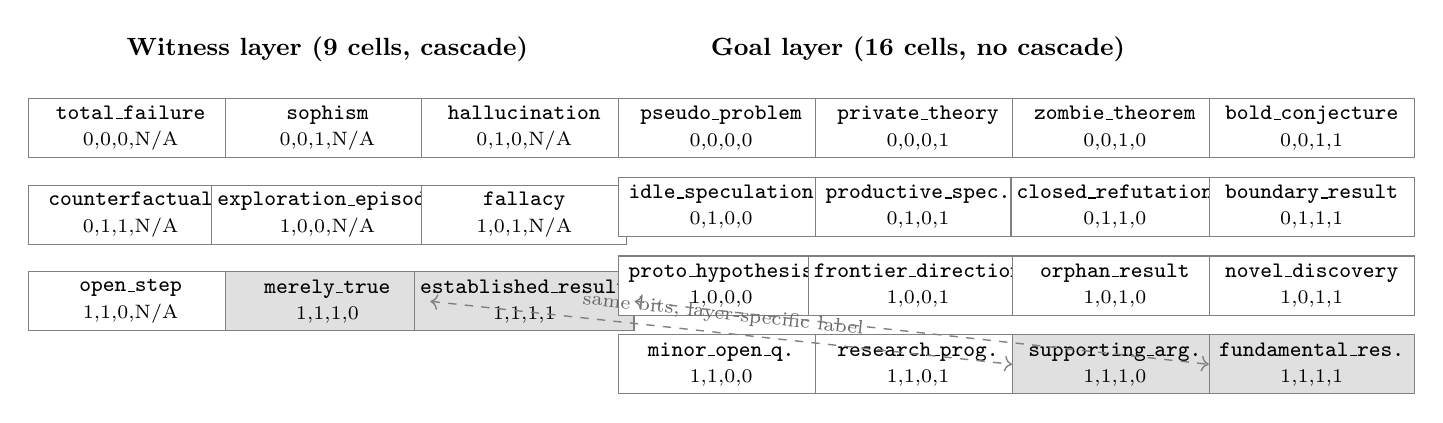
\begin{tikzpicture}[
  font=\footnotesize,
  cell/.style={
    rectangle, draw=black!50, fill=white,
    minimum width=2.6cm, minimum height=0.75cm, align=center,
    inner sep=2pt
  },
  cellgray/.style={
    cell, fill=black!12
  },
  bits/.style={font=\scriptsize\ttfamily, black!70},
  hdr/.style={font=\small\bfseries},
]

% Witness layer (left, 9 cells in a 3x3 grid + 2 highlighted bottom)
\node[hdr] at (-3.5, 4) {Witness layer (9 cells, cascade)};

\node[cell] (w1) at (-6, 3) {\texttt{total\_failure}\\{\scriptsize 0,0,0,N/A}};
\node[cell] (w2) at (-3.5, 3) {\texttt{sophism}\\{\scriptsize 0,0,1,N/A}};
\node[cell] (w3) at (-1, 3) {\texttt{hallucination}\\{\scriptsize 0,1,0,N/A}};
\node[cell] (w4) at (-6, 1.9) {\texttt{counterfactual}\\{\scriptsize 0,1,1,N/A}};
\node[cell] (w5) at (-3.5, 1.9) {\texttt{exploration\_episode}\\{\scriptsize 1,0,0,N/A}};
\node[cell] (w6) at (-1, 1.9) {\texttt{fallacy}\\{\scriptsize 1,0,1,N/A}};
\node[cell] (w7) at (-6, 0.8) {\texttt{open\_step}\\{\scriptsize 1,1,0,N/A}};
\node[cellgray] (w8) at (-3.5, 0.8) {\texttt{merely\_true}\\{\scriptsize 1,1,1,0}};
\node[cellgray] (w9) at (-1, 0.8) {\texttt{established\_result}\\{\scriptsize 1,1,1,1}};

% Goal layer (right, 16 cells in 4x4)
\node[hdr] at (4, 4) {Goal layer (16 cells, no cascade)};

\node[cell] (g1A) at (1.5, 3.0) {\texttt{pseudo\_problem}\\{\scriptsize 0,0,0,0}};
\node[cell] (g1B) at (4.0, 3.0) {\texttt{private\_theory}\\{\scriptsize 0,0,0,1}};
\node[cell] (g2A) at (6.5, 3.0) {\texttt{zombie\_theorem}\\{\scriptsize 0,0,1,0}};
\node[cell] (g2B) at (9.0, 3.0) {\texttt{bold\_conjecture}\\{\scriptsize 0,0,1,1}};

\node[cell] (g3A) at (1.5, 2.0) {\texttt{idle\_speculation}\\{\scriptsize 0,1,0,0}};
\node[cell] (g3B) at (4.0, 2.0) {\texttt{productive\_spec.}\\{\scriptsize 0,1,0,1}};
\node[cell] (g4A) at (6.5, 2.0) {\texttt{closed\_refutation}\\{\scriptsize 0,1,1,0}};
\node[cell] (g4B) at (9.0, 2.0) {\texttt{boundary\_result}\\{\scriptsize 0,1,1,1}};

\node[cell] (g5A) at (1.5, 1.0) {\texttt{proto\_hypothesis}\\{\scriptsize 1,0,0,0}};
\node[cell] (g5B) at (4.0, 1.0) {\texttt{frontier\_direction}\\{\scriptsize 1,0,0,1}};
\node[cell] (g6A) at (6.5, 1.0) {\texttt{orphan\_result}\\{\scriptsize 1,0,1,0}};
\node[cell] (g6B) at (9.0, 1.0) {\texttt{novel\_discovery}\\{\scriptsize 1,0,1,1}};

\node[cell] (g7A) at (1.5, 0.0) {\texttt{minor\_open\_q.}\\{\scriptsize 1,1,0,0}};
\node[cell] (g7B) at (4.0, 0.0) {\texttt{research\_prog.}\\{\scriptsize 1,1,0,1}};
\node[cellgray] (g8) at (6.5, 0.0) {\texttt{supporting\_arg.}\\{\scriptsize 1,1,1,0}};
\node[cellgray] (g9) at (9.0, 0.0) {\texttt{fundamental\_res.}\\{\scriptsize 1,1,1,1}};

% Specialization annotation between layers
\draw[<->, dashed, black!50, line width=0.5pt]
  (w8.east) -- node[font=\scriptsize, midway, above, sloped, black!60]
    {same bits, layer-specific label} (g8.west);
\draw[<->, dashed, black!50, line width=0.5pt]
  (w9.east) -- node[font=\scriptsize, midway, above, sloped, black!60]
    {} (g9.west);

\end{tikzpicture}
\caption{The locked verdict-bits to cell-label assembly mapping. Witness layer
(left, 9 cells): cascade collapses 7 of 16 verdict vectors to $\text{Inv}=\text{N/A}$;
the remaining 9 cells are named by the witness-layer interpretation of each
gate. Goal layer (right, 16 cells): all four gates fire independently, so
the full $2^4$ verdict space is named.
The two cells highlighted in each layer share verdict bits with their counterparts
in the other layer (the dashed two-headed arrows): $(1,1,1,0)$ is
\texttt{merely\_true} as a witness but \texttt{supporting\_argument} as a goal;
$(1,1,1,1)$ is \texttt{established\_result} as a witness but
\texttt{fundamental\_result} as a goal. This is specialization-at-instance,
not a violation of gate-invariance.}
\label{fig:cell_taxonomy}
\end{figure}

% Witness-layer cascade rule illustration.
% Designed for single column.
\begin{figure}[t]
\centering
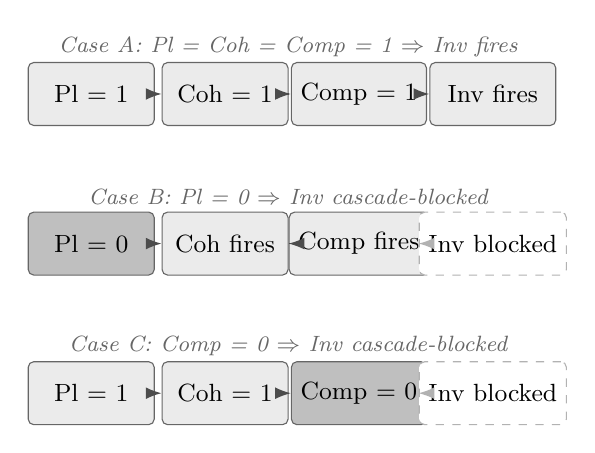
\begin{tikzpicture}[
  font=\small,
  gate/.style={
    rectangle, rounded corners=2pt,
    minimum width=1.6cm, minimum height=0.8cm, align=center,
    draw=black!60
  },
  pass/.style={fill=black!8},
  fail/.style={fill=black!25},
  blocked/.style={fill=white, draw=black!30, dashed},
  arrow/.style={-{Latex[length=2mm]}, black!70, line width=0.5pt},
  blockarrow/.style={-{Latex[length=2mm]}, black!30, line width=0.5pt, dashed},
  caselabel/.style={font=\footnotesize\itshape, black!60},
]

% Case A: Pl=Coh=Comp=1, Inv fires
\node[caselabel] at (3.5, 4.6) {Case A: Pl = Coh = Comp = 1 $\Rightarrow$ Inv fires};
\node[gate, pass] (a_pl)   at (1.0, 4.0) {Pl = 1};
\node[gate, pass] (a_coh)  at (2.7, 4.0) {Coh = 1};
\node[gate, pass] (a_comp) at (4.4, 4.0) {Comp = 1};
\node[gate, pass] (a_inv)  at (6.1, 4.0) {Inv fires};
\draw[arrow] (a_pl.east)   -- (a_coh.west);
\draw[arrow] (a_coh.east)  -- (a_comp.west);
\draw[arrow] (a_comp.east) -- (a_inv.west);

% Case B: Pl=0 -> Inv blocked
\node[caselabel] at (3.5, 2.7) {Case B: Pl = 0 $\Rightarrow$ Inv cascade-blocked};
\node[gate, fail] (b_pl)    at (1.0, 2.1) {Pl = 0};
\node[gate, pass] (b_coh)   at (2.7, 2.1) {Coh fires};
\node[gate, pass] (b_comp)  at (4.4, 2.1) {Comp fires};
\node[gate, blocked] (b_inv) at (6.1, 2.1) {Inv blocked};
\draw[arrow] (b_pl.east)    -- (b_coh.west);
\draw[arrow] (b_coh.east)   -- (b_comp.west);
\draw[blockarrow] (b_comp.east) -- (b_inv.west);

% Case C: Comp=0 -> Inv blocked
\node[caselabel] at (3.5, 0.8) {Case C: Comp = 0 $\Rightarrow$ Inv cascade-blocked};
\node[gate, pass] (c_pl)    at (1.0, 0.2) {Pl = 1};
\node[gate, pass] (c_coh)   at (2.7, 0.2) {Coh = 1};
\node[gate, fail] (c_comp)  at (4.4, 0.2) {Comp = 0};
\node[gate, blocked] (c_inv) at (6.1, 0.2) {Inv blocked};
\draw[arrow] (c_pl.east)    -- (c_coh.west);
\draw[arrow] (c_coh.east)   -- (c_comp.west);
\draw[blockarrow] (c_comp.east) -- (c_inv.west);

\end{tikzpicture}
\caption{Witness-layer cascade rule. Plausibility, Coherence, and
Completeness fire independently. Invariance fires only if all three
prerequisites pass (Case~A). When any prerequisite fails, Invariance is
\emph{cascade-blocked}: \texttt{fired = false},
\texttt{verdict = null}, \texttt{fired\_false\_reason = cascade\_blocked}.
The cascade is asymmetric across layers --- the goal layer has no cascade,
which is the source of the difference in cell counts (9 vs 16).}
\label{fig:cascade}
\end{figure}

% Witness-loop iterative re-evaluation mechanism.
% Designed for single column.
\begin{figure}[t]
\centering
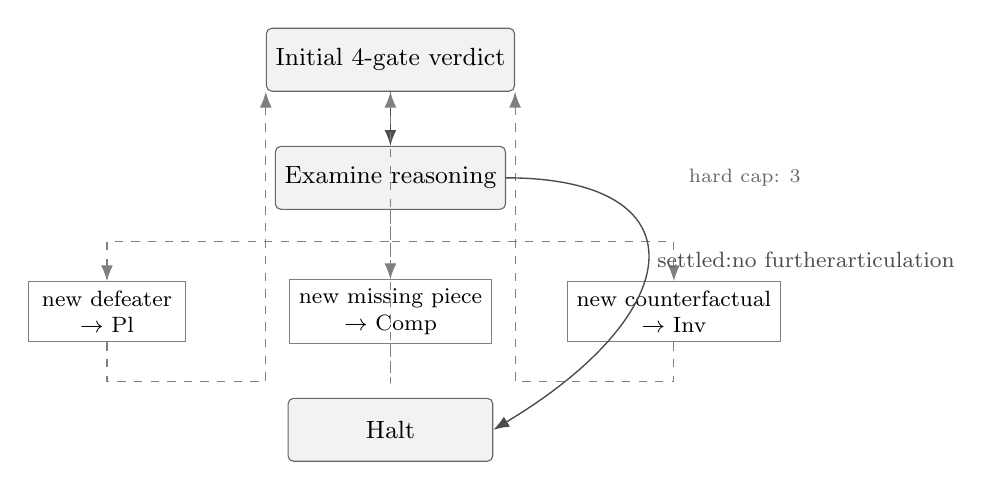
\begin{tikzpicture}[
  font=\small,
  block/.style={
    rectangle, rounded corners=2pt, draw=black!60, fill=black!5,
    minimum width=2.6cm, minimum height=0.8cm, align=center
  },
  routebox/.style={
    rectangle, draw=black!50, fill=white,
    minimum width=2.0cm, minimum height=0.6cm, align=center,
    font=\footnotesize
  },
  arrow/.style={-{Latex[length=2mm]}, black!70, line width=0.5pt},
  routearrow/.style={-{Latex[length=2mm]}, black!50, line width=0.4pt, dashed},
]

% Initial verdict
\node[block] (init) at (0, 3.0) {Initial 4-gate verdict};

% Iterate decision
\node[block] (iter) at (0, 1.5) {Examine reasoning};

% Three routes back
\node[routebox] (newpl)   at (-3.6, -0.2) {new defeater\\$\to$ Pl};
\node[routebox] (newcomp) at (0,    -0.2) {new missing piece\\$\to$ Comp};
\node[routebox] (newinv)  at (3.6,  -0.2) {new counterfactual\\$\to$ Inv};

% Halt
\node[block] (halt) at (0, -1.7) {Halt};

% Cap
\node[font=\scriptsize, black!60] at (4.5, 1.5) {hard cap: 3};

% Flows
\draw[arrow] (init.south) -- (iter.north);
\draw[routearrow] (iter.south) -- ++(0,-0.4) -| (newpl.north);
\draw[routearrow] (iter.south) -- (newcomp.north);
\draw[routearrow] (iter.south) -- ++(0,-0.4) -| (newinv.north);

\draw[routearrow] (newpl.south)   |- ++(0, -0.5) -| (init.south west);
\draw[routearrow] (newcomp.south) |- ++(0, -0.5) -| (init.south);
\draw[routearrow] (newinv.south)  |- ++(0, -0.5) -| (init.south east);

\draw[arrow] (iter.east) .. controls +(2.5,0) and +(2.5,1.5) .. (halt.east)
  node[midway, right, font=\footnotesize, black!70]
  {settled: \\ no further \\ articulation};

\end{tikzpicture}
\caption{Witness-loop re-evaluation mechanism. After each round of gate
verdicts, the judge inspects its own reasoning for new evidence: a new
defeater routes back to Plausibility; a new missing piece to Completeness;
a new counterfactual to Invariance. Iterations are capped at 3; most cases
halt at iteration~1 with \texttt{halt\_reason} = \texttt{no\_further\_articulation}.
This mechanic supports the rubric's recursive observer principle ---
the reviewer is inside the evaluative loop and routes new evidence back
to the relevant gate rather than collapsing to a single-pass verdict.}
\label{fig:witness_loop}
\end{figure}

% Goal-witness alignment failure schematic, using AS-v2 compositional regularization
% as the canonical case study. Designed for full text-width.
\begin{figure}[t]
\centering
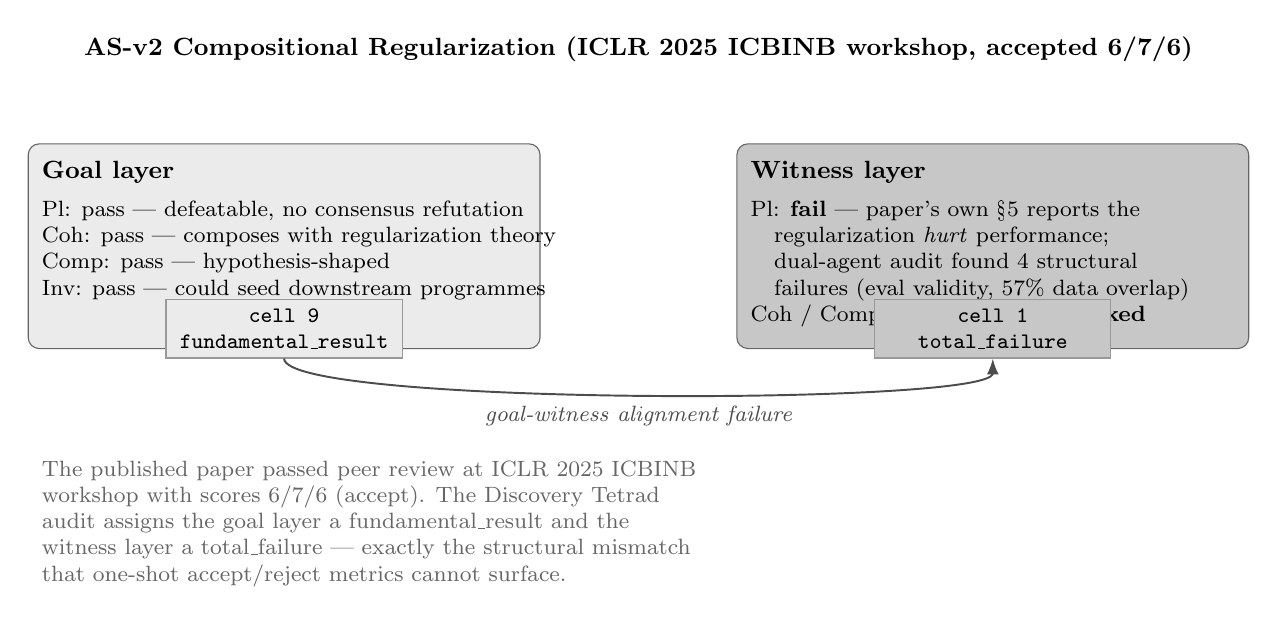
\begin{tikzpicture}[
  font=\small,
  layer/.style={
    rectangle, rounded corners=4pt, draw=black!60,
    minimum width=6.5cm, minimum height=2.6cm, align=left
  },
  pass/.style={fill=black!8},
  fail/.style={fill=black!22},
  cellbox/.style={
    rectangle, draw=black!40, fill=white,
    minimum width=3.0cm, minimum height=0.7cm, align=center,
    font=\footnotesize\ttfamily
  },
  goalcell/.style={cellbox, fill=black!8},
  witcell/.style={cellbox, fill=black!22},
  arrow/.style={-{Latex[length=2mm]}, black!70, line width=0.5pt},
]

% Headline panel
\node[font=\small\bfseries] at (4.5, 5.5)
  {AS-v2 Compositional Regularization (ICLR 2025 ICBINB workshop, accepted 6/7/6)};

% Goal layer panel (left)
\node[layer, pass] (goal) at (0, 3) {};
\node[font=\small\bfseries, anchor=north west] at (-3.2, 4.2) {Goal layer};
\node[align=left, font=\footnotesize, anchor=north west] at (-3.2, 3.7)
  {Pl: pass --- defeatable, no consensus refutation \\
   Coh: pass --- composes with regularization theory \\
   Comp: pass --- hypothesis-shaped \\
   Inv: pass --- could seed downstream programmes};
\node[goalcell] (gc) at (0, 1.95) {cell 9 \\ fundamental\_result};

% Witness layer panel (right)
\node[layer, fail] (wit) at (9, 3) {};
\node[font=\small\bfseries, anchor=north west] at (5.8, 4.2) {Witness layer};
\node[align=left, font=\footnotesize, anchor=north west] at (5.8, 3.7)
  {Pl: \textbf{fail} --- paper's own \S5 reports the \\
   \quad regularization \emph{hurt} performance; \\
   \quad dual-agent audit found 4 structural \\
   \quad failures (eval validity, 57\% data overlap) \\
   Coh / Comp / Inv: \textbf{cascade-blocked}};
\node[witcell] (wc) at (9, 1.95) {cell 1 \\ total\_failure};

% Connection: same artifact, two layers
\draw[arrow, line width=0.7pt]
  (gc.south) .. controls +(0,-0.6) and +(0,-0.6) .. (wc.south);
\node[font=\footnotesize\itshape, black!70] at (4.5, 0.85)
  {goal-witness alignment failure};

% Comparison annotation
\node[align=left, font=\footnotesize, anchor=north west, black!60] at (-3.2, 0.4)
  {The published paper passed peer review at ICLR 2025 ICBINB \\
   workshop with scores 6/7/6 (accept). The Discovery Tetrad \\
   audit assigns the goal layer a fundamental\_result and the \\
   witness layer a total\_failure --- exactly the structural mismatch \\
   that one-shot accept/reject metrics cannot surface.};

\end{tikzpicture}
\caption{The canonical \emph{goal-witness alignment failure} pattern, illustrated
on the AS-v2 Compositional Regularization paper. The audit cleanly separates
the goal --- a coherent, defeatable, hypothesis-shaped, foundational
research target --- from the witness, which fails on plausibility once the
paper's own results are read carefully. The cascade rule then blocks the
remaining gates. Peer review at ICLR 2025 ICBINB scored the paper 6/7/6
(accept); the rubric registers the structural mismatch the headline metric
hides.}
\label{fig:goal_witness_failure}
\end{figure}

% Sophism density per goal across substrates (the headline discriminative axis).
% Uses pgfplots. Designed for full text-width or single column.
\begin{figure}[t]
\centering
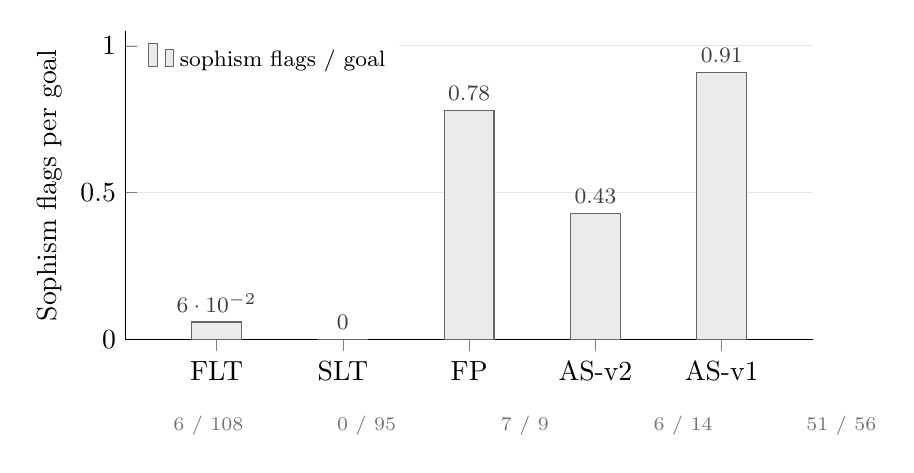
\begin{tikzpicture}
\begin{axis}[
  width=0.85\textwidth,
  height=5.5cm,
  ybar,
  bar width=18pt,
  enlarge x limits=0.18,
  ymin=0,
  ymax=1.05,
  ylabel={Sophism flags per goal},
  xlabel={},
  symbolic x coords={FLT, SLT, FP, AS-v2, AS-v1},
  xtick=data,
  nodes near coords,
  nodes near coords style={font=\footnotesize},
  ymajorgrids,
  major grid style={black!10},
  axis lines*=left,
  tick style={black!50},
  every node near coord/.append style={font=\footnotesize, color=black!75},
  legend style={
    at={(0.02,0.98)},
    anchor=north west,
    draw=none,
    fill=white,
    font=\footnotesize,
  },
]
\addplot[fill=black!8, draw=black!60] coordinates {
  (FLT, 0.06)
  (SLT, 0.00)
  (FP, 0.78)
  (AS-v2, 0.43)
  (AS-v1, 0.91)
};
\addlegendentry{sophism flags / goal}

\end{axis}

% Absolute-count annotations below the x-axis labels (in tikzpicture coords).
\node[font=\scriptsize, anchor=north, black!55] at (1.05, -0.85) {6 / 108};
\node[font=\scriptsize, anchor=north, black!55] at (3.06, -0.85) {0 / 95};
\node[font=\scriptsize, anchor=north, black!55] at (5.07, -0.85) {7 / 9};
\node[font=\scriptsize, anchor=north, black!55] at (7.08, -0.85) {6 / 14};
\node[font=\scriptsize, anchor=north, black!55] at (9.09, -0.85) {51 / 56};
\end{tikzpicture}
\caption{Sophism flag density across the five substrates. The two
pre-verified-clean Lean substrates (FLT, SLT) sit near zero. The two
autonomous-AI-generated paper substrates (AS-v1, AS-v2) and the public
mathematical research benchmark (FP) sit substantially higher. Counts shown
below each bar are flagged records over total goal records.
The discriminative gap (Lean substrates: 6 sophism flags over 203 goals,
0.03/goal; AS papers: 57 over 70, 0.81/goal) is approximately 27$\times$ ---
the rubric resolves the substrates that the headline accept/reject metric
cannot.}
\label{fig:sophism_density}
\end{figure}

% Cell-occupancy heatmap: substrate x cell counts at goal layer.
% Pure TikZ matrix (no pgfplots) so the annotation logic is robust.
% Designed for full text-width.
\begin{figure}[t]
\centering
\begin{tikzpicture}[
  font=\footnotesize,
  cell/.style={
    rectangle, draw=black!30, line width=0.3pt,
    minimum width=0.8cm, minimum height=0.6cm, align=center,
    inner sep=0pt
  },
]

% Cell list (16 columns)
\def\cells{1A,1B,2A,2B,3A,3B,4A,4B,5A,5B,6A,6B,7A,7B,8,9}
% Substrates (5 rows, top to bottom)
\def\substrates{FLT,SLT,FP,AS-v2,AS-v1}

% Counts data: row major.
% Order: FLT, SLT, FP, AS-v2, AS-v1.
% Cells: 1A 1B 2A 2B 3A 3B 4A 4B 5A 5B 6A 6B 7A 7B 8 9
% (zero entries shown as empty cells)
\def\dataFLT{0,0,2,0,0,0,3,0,0,0,0,1,2,0,7,93}
\def\dataSLT{0,0,0,0,0,0,0,0,0,0,0,0,0,0,17,78}
\def\dataFP{0,0,0,0,0,0,0,1,0,0,0,0,0,0,0,8}
\def\dataASvtwo{0,0,0,0,0,0,2,0,0,0,0,0,0,1,4,7}
\def\dataASvone{0,0,4,0,4,0,3,1,1,0,0,0,0,3,6,34}

% Header row: cell ids
\foreach \c [count=\i from 0] in 1A,1B,2A,2B,3A,3B,4A,4B,5A,5B,6A,6B,7A,7B,8,9 {
  \node[font=\scriptsize, black!70] at (\i*0.8 + 0.4, 0.7) {\c};
}

% Substrate row labels
\foreach \s [count=\j from 0] in FLT, SLT, FP, AS-v2, AS-v1 {
  \node[font=\scriptsize\bfseries, anchor=east] at (-0.1, -\j*0.6) {\s};
}

% FLT row
\foreach \v [count=\i from 0] in 0,0,2,0,0,0,3,0,0,0,0,1,2,0,7,93 {
  \pgfmathtruncatemacro{\shade}{min(75, \v)}
  \node[cell, fill=black!\shade] at (\i*0.8 + 0.4, 0) {%
    \ifnum\v>0\textcolor{black!90}{\v}\fi};
}
% SLT row
\foreach \v [count=\i from 0] in 0,0,0,0,0,0,0,0,0,0,0,0,0,0,17,78 {
  \pgfmathtruncatemacro{\shade}{min(75, \v)}
  \node[cell, fill=black!\shade] at (\i*0.8 + 0.4, -0.6) {%
    \ifnum\v>0\textcolor{black!90}{\v}\fi};
}
% FP row
\foreach \v [count=\i from 0] in 0,0,0,0,0,0,0,1,0,0,0,0,0,0,0,8 {
  \pgfmathtruncatemacro{\shade}{min(75, \v*8)}
  \node[cell, fill=black!\shade] at (\i*0.8 + 0.4, -1.2) {%
    \ifnum\v>0\textcolor{black!90}{\v}\fi};
}
% AS-v2 row
\foreach \v [count=\i from 0] in 0,0,0,0,0,0,2,0,0,0,0,0,0,1,4,7 {
  \pgfmathtruncatemacro{\shade}{min(75, \v*8)}
  \node[cell, fill=black!\shade] at (\i*0.8 + 0.4, -1.8) {%
    \ifnum\v>0\textcolor{black!90}{\v}\fi};
}
% AS-v1 row
\foreach \v [count=\i from 0] in 0,0,4,0,4,0,3,1,1,0,0,0,0,3,6,34 {
  \pgfmathtruncatemacro{\shade}{min(75, \v*2)}
  \node[cell, fill=black!\shade] at (\i*0.8 + 0.4, -2.4) {%
    \ifnum\v>0\textcolor{black!90}{\v}\fi};
}

% Axis labels
\node[font=\small\bfseries] at (6.4, 1.4) {Goal-layer cell};

\end{tikzpicture}
\caption{Goal-layer cell-occupancy across the five substrates (282 records,
counts shown). FLT and SLT concentrate in cell~9 (\texttt{fundamental\_result})
with a small tail in cell~8 (\texttt{supporting\_argument}). The AS-v1 and
AS-v2 substrates spread across cells 2A, 3A, 4A, 7B, 8, and 9 --- the
failure-mode cells the rubric exists to resolve. The First-Proof substrate
(FP) sits intermediate, with strong cell-9 occupancy and one cell-4B
(\texttt{boundary\_result}) entry on Problem~5. Empty cells are zero;
darker cells carry larger counts.}
\label{fig:cell_heatmap}
\end{figure}

% Three-way concordance: Claude / GPT / Human on the FP subset.
% Schematic for the inter-judge concordance appendix.
\begin{figure}[t]
\centering
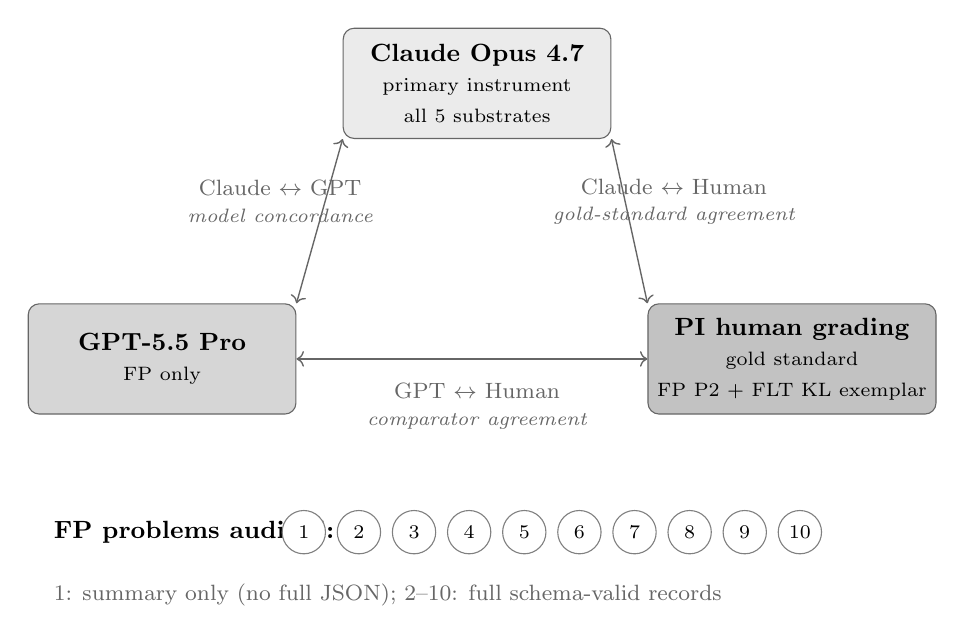
\begin{tikzpicture}[
  font=\small,
  judge/.style={
    rectangle, rounded corners=4pt, draw=black!60,
    minimum width=3.4cm, minimum height=1.4cm, align=center
  },
  jclaude/.style={judge, fill=black!8},
  jgpt/.style={judge, fill=black!16},
  jhuman/.style={judge, fill=black!24},
  arrow/.style={-{Latex[length=2mm]}, black!70, line width=0.5pt},
  pair/.style={<->, black!60, line width=0.5pt},
  prob/.style={
    circle, draw=black!50, fill=white,
    minimum size=0.55cm, font=\scriptsize, inner sep=0pt
  },
]

% Three judges arranged as a triangle
\node[jclaude] (claude) at (0, 3.5)
  {\textbf{Claude Opus 4.7}\\\scriptsize primary instrument\\\scriptsize all 5 substrates};
\node[jgpt] (gpt) at (-4, 0)
  {\textbf{GPT-5.5 Pro}\\\scriptsize FP only};
\node[jhuman] (human) at (4, 0)
  {\textbf{PI human grading}\\\scriptsize gold standard\\\scriptsize FP P2 + FLT KL exemplar};

% Pairwise comparisons
\draw[pair] (claude.south west) -- (gpt.north east);
\draw[pair] (claude.south east) -- (human.north west);
\draw[pair] (gpt.east) -- (human.west);

% Pair labels
\node[font=\footnotesize, black!60, align=center] at (-2.5, 2.0)
  {Claude $\leftrightarrow$ GPT \\ \scriptsize\itshape model concordance};
\node[font=\footnotesize, black!60, align=center] at (2.5, 2.0)
  {Claude $\leftrightarrow$ Human \\ \scriptsize\itshape gold-standard agreement};
\node[font=\footnotesize, black!60, align=center] at (0, -0.6)
  {GPT $\leftrightarrow$ Human \\ \scriptsize\itshape comparator agreement};

% Per-problem strip below
\node[font=\small\bfseries, anchor=west] at (-5.5, -2.2) {FP problems audited:};
\foreach \i/\x in {1/-2.2, 2/-1.5, 3/-0.8, 4/-0.1, 5/0.6, 6/1.3, 7/2.0, 8/2.7, 9/3.4, 10/4.1} {
  \node[prob] at (\x, -2.2) {\i};
}
\node[font=\footnotesize, anchor=west, black!60] at (-5.5, -3.0)
  {1: summary only (no full JSON); 2--10: full schema-valid records};

\end{tikzpicture}
\caption{Three-way inter-judge concordance design for the First-Proof subset.
The Discovery Tetrad audit's primary instrument is Claude Opus 4.7, applied
uniformly to all five substrates. To measure inter-judge reliability, the
First-Proof problems were also independently audited by GPT-5.5 Pro and
graded by hand by the authors using a structured exemplar protocol. The
three pairwise agreement statistics (Claude $\leftrightarrow$ GPT,
Claude $\leftrightarrow$ Human, GPT $\leftrightarrow$ Human) populate the
concordance appendix; the human grade is treated as the gold standard.
Problem~1 has only a Markdown summary (no full structured JSON) on the
GPT-judge side; Problems 2--10 carry full schema-valid records.}
\label{fig:concordance}
\end{figure}


\end{document}
